% \chapter{Evaluation} 
% The project had 2 aspects to evaluate- the TML and the product (website). Both aspects were evaluated continually through unit tests during production and tested using a user evaluation.

% After the product had been completed, a user evaluation was conducted on 18 second year computing students. TMs are taught to students that have few years of programming experience, and for this reason second years were chosen. They had little familiarity, if any, with Turing Machines and were introduced to both TMs and TML during the evaluation session. 

% The aim of the evaluation was for them to get acquainted with TMs and TML programs, and then to:
% \begin{itemize}
%     \item compare TMs and TML programs;
%     \item understand whether writing a TML program would help drawing a TM; and
%     \item evaluate the product.
% \end{itemize}
% The evaluation session also served as a great opportunity to ask for any features to be added to the product and the language.

% During the evaluation session, students were first introduced to TML programs. They were then expected to understand what language two mystery TML programs accept. They were expected to do so by checking whether the programs accepted some values. During this process, they should have been able understand the way the program operates and decode the language it accepts. They were expected to use the product to help them follow the code and understand the steps in execution. 

% The students were then introduced to TMs, and expected to decode 2 TMs in a similar manner. Since the website can only execute TML programs, they were given TML programs for the TM. Note however that this did not defeat the purpose of testing TMs since the programs given were complete TML programs, which is essentially another representation for TMs.

% Finally, they were asked to write some programs in the TML. Like in the previous sections, they were free to use the website to write the programs and test its correctness. The first few programs were quite similar to the code they had seen before. The remaining programs were somewhat more difficult, and for this reason they were optional. Nonetheless, many students attempted them and wrote impressive programs! 
% % TODO: think-aloud methodology

% The evaluation took about 50 minutes to be completed. The students were asked to fill out a worksheet with their answers. 

% After they had completed the worksheet, they completed a survey to evaluate the language and the product. To avoid writing programs on paper, students were asked to copy their code from the final part of the worksheet to the survey. The results of the survey are discussed in detail in the next section. Both the worksheet and the survey are given in the appendix. 

% \section{Evaluation Results}
% \subsection{Parser and Language Evaluation}
% The parser was continually tested during production to ensure correctness. This was achieved using unit testing. They were used to test all aspects of the parser and were extensive. In fact, the unit tests had more than $95\%$ code coverage.

% \begin{figure}[htb]
%     \centering
%     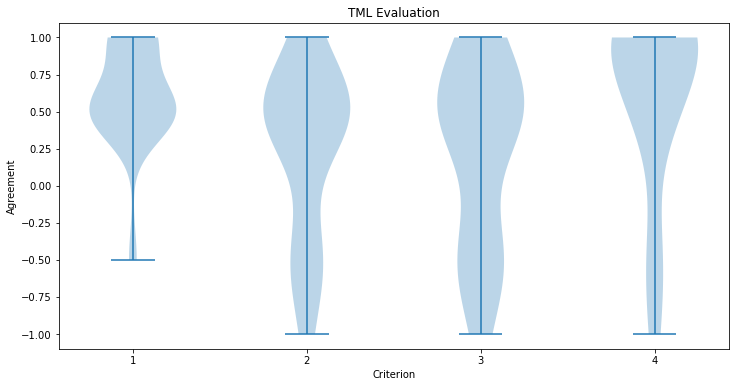
\includegraphics[scale=0.35]{images/tml-evaluation.png}
%     \caption{A violin plot that summarises the results of the survey relating to the TML with respect to the 4 criteria. The agreement value refers to how much the user agrees to the statement: $-1$ is strongly disagree; $-0.5$ disagree; $0.5$ agree and $1$ strongly agree. The whiskers show the range of answers, e.g. nobody said they strongly disagreed with criterion 1. Moreover, the density is proportional to the number of participants answering the question with that value, e.g. most people answered criterion 1 with the value $0.5$ (agree).}
%     \label{fig:tml-evaluation}
% \end{figure}

% During user evaluation, users were asked to evaluate the language in the following criteria:
% \begin{enumerate}
%     \item TML is easy to understand
%     \item TML is easy to write programs in
%     \item I was able to fix errors in my code using the error messages provided
%     \item I was able to easily reason executing a program on a tape
% \end{enumerate}
% They were asked to rate how much they agreed with each statement, and the result is summarised for each criterion in Figure \ref{fig:tml-evaluation}. 

% It is clear that most students found the language easy to understand. Students noted that the syntax is quite similar to Java, a language they are quite familiar with. It is also clear from the worksheet solutions that the language is easy to follow- most students were able to correctly identify and explain which values a TML program accepts.

% However, a smaller number of students believed that the language is easy to write programs in- the solutions to the worksheet illustrate that some students found it harder to write (syntactically) correct programs than to understand it. This is expected given that they were only exposed to the language for about an hour.

% Many found the error messages quite useful and it helped them write correct programs, but few disagreed with this. A student mentioned that some of the error messages could have been given more details, for example a missing case error did not identify what letter in the case was missing. This issue was fixed after the evaluation sessions- now, the missing letter is mentioned in the error message.

% Most students found it easy to reason executing a program on a tape- they were able to run the code on the website and follow the code quite easily. Since the students were not formally introduced to the language, some of the students struggled to reason execution of the code they had written. For instance, consider the following block of code:
% \begin{lstlisting}[language=TML]
% if a {
%     changeto blank
%     goto someModule
% }
% \end{lstlisting}
% When this code is executed, and the tapehead value is \texttt{a}, the value gets changed to \texttt{blank} as expected. However, the tape also moves to the \texttt{left} before moving to the module \texttt{someModule}. This is the default behaviour, but the students were not informed of this. If there was more time for evaluation, the rules of execution would have been explained more thoroughly. Nonetheless, by asking the students to explicitly include the commands, this issue was partially mitigated.

% \begin{figure}[htb]
%     \centering
%     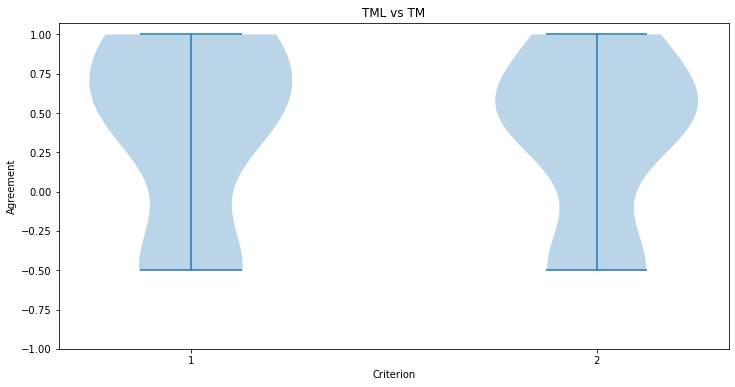
\includegraphics[scale=0.35]{images/tml-v-tm.png}
%     \caption{A violin plot that summarises the results of the survey that compare TM and TML with respect to the 2 criteria.}
%     \label{fig:tml-v-tm}
% \end{figure}

% The TML was then directly compared to TMs. In particular, students were asked to compare TMs and TML programs in the following criteria:
% \begin{enumerate}
%     \item I am more confident in writing a program in TML than drawing a TM
%     \item I find it easier to reason what a TML program accepts than a TM
% \end{enumerate}
% The students were asked to rate how much they agreed with each statement, and the result is summarised for the two criteria in Figure \ref{fig:tml-v-tm}. 

% Overall, students seem to be more comfortable with TML than TM. They were more confident writing a TML than drawing a TM- this is expected since they were not asked to draw a TM. From the worksheet, it is evident that students were able to replicate the code given and write correct programs, and to a lesser extent, devise new programs.

% It is somewhat surprising that many found it easier to reason a TML program than a TM. This is because many claimed that it is easier to follow the TM diagram than code. Nonetheless, the students might have found it easier to reason a TML program since the worksheet focuses much more on TML than TM.
% % TODO: Some sort of bias- research?

% \begin{figure}[htb]
%     \centering
%     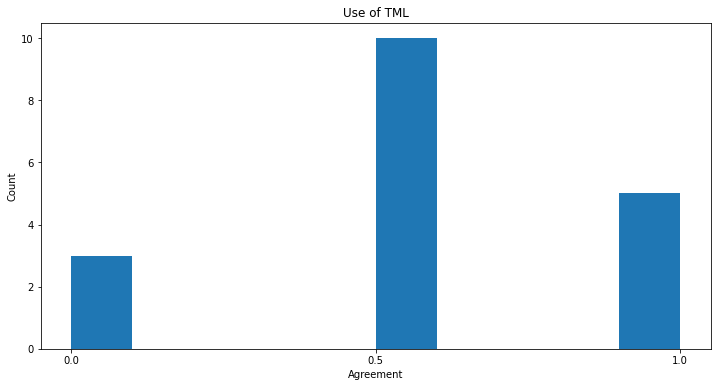
\includegraphics[scale=0.35]{images/use-tml.png}
%     \caption{A histogram that summarises whether the users would consider writing a TML program before drawing a TM. 0 means no; 0.5 means maybe; and 1 means yes.}
%     \label{fig:use-tml}
% \end{figure}

% The students were then asked whether they would consider writing a TML program before drawing a TM. The response of this question is summarised in Figure \ref{fig:use-tml}. 

% When drawing a TM for some algorithm, it is quite helpful to plan the machine beforehand. TML provides an opportunity where it is possible to reason in quite low-level how the algorithm is meant to execute on a tape without considering the states and transitions in a TM. Moreover, it is quite easy to convert a TML to a TM. I believe this is the main selling point of the language. 

% From the results, it is clear that many would consider drawing it. The hesitation might result from the little experience that they had gotten. Moreover, most students only attempted questions involving simple algorithms. Nonetheless, the few students that attempted the harder questions exclaimed that they would struggle directly drawing a TM for those algorithms.

% In summary, the TML language seems to be a promising alternative to TMs. Due to the short length and small number of participants of the evaluation, it cannot be concluded whether it is easier to learn about TMs using FMs or through TML programs. Nonetheless, it seems that TML programs are relatively easy to learn and understand. Further evaluation would help compare it more thoroughly with TMs and explore the true potential of the language.

% \subsection{Product Evaluation}
% Like with the language, the product was also continually tested during production for correctness. This was achieved through unit testing. Unlike the testing for language, this was however less successful due to the limits in mocking frameworks and time constraints. Nonetheless, the tests covered all the major parts of the website and ensured that all the functionalities implemented were correct. If there was more time, the mocking would be more thorough so that the tests could be exhaustive.

% % This was because of the use of frameworks in the website. They were mocked during testing, so all the functionalities they provide could not be tested completely.

% During the user evaluation, the students were expected to use the product to understand TMLs and TMs. For this reason, they were able to evaluate the website. In the survey, they were asked to evaluate the product in the following 7 criteria:
% % Note that only the homepage could be evaluated; the documentation was not evaluated since I directly explained how the TML programs and TMs work. 
% \begin{enumerate}
%     \item The website is easy to follow
%     \item The presentation of the website is intuitive
%     \item There were no visible bugs in the website
%     \item The website was fast
%     \item The website feels complete
%     \item The code execution was easy to follow
%     \item The code editor was easy to use
% \end{enumerate}
% The results of the survey are summarised in Figure \ref{fig:website-evaluation}. 

% \begin{figure}[htb]
%     \centering
%     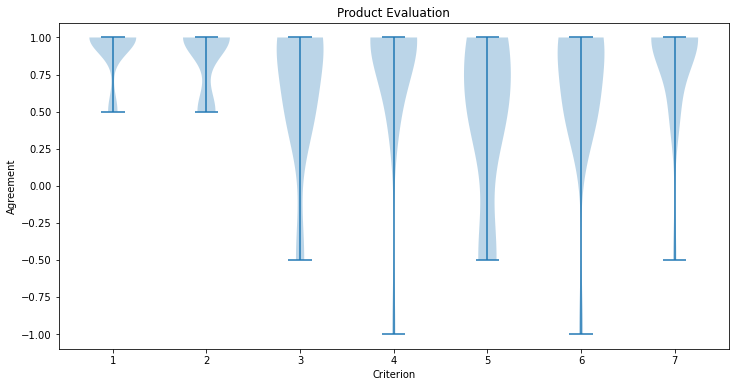
\includegraphics[scale=0.35]{images/website-evaluation.png}
%     \caption{A violin plot that summarises the results of the survey relating to the website with respect to the 7 criteria.}
%     \label{fig:website-evaluation}
% \end{figure}

% It is evident that most found the website easy to follow and intuitive to use. Unfortunately, there were a few bugs present, e.g. the TM did not change to the latest version when tape execution began. These bugs were fixed later after the evaluation sessions. Most also found the website to be fast and complete. 

% Some did not find code execution easy to follow- this was particularly the case with long programs where students had to scroll to find the currently executing block of code. Also, some found the code editor difficult to use. There were some issues in using the code editor- the code cannot be edited while being executed, but there was no feedback to inform the user about this issue. A pop-up has now been added to warn them of this issue.

% Overall, it is clear that the website serves as a good platform to parse a TML program and execute it on a tape. There are still some issues with the website that can be fixed later. Nonetheless, the website feels complete and functions as expected.

% \section{Limitations to Evaluation}
% Due to the time constraints of the project, there were some limitations to the evaluation, in particular the user evaluation. The biggest limitation was the length of the evaluation session. It was hard to conduct a productive, short and accessible session. 
% % In fact, the first evaluation session took considerably longer than an hour, after which I made substantial changes to the questions (i.e. made some easier and some others optional) to ensure that it fits within an hour!

% For this reason, it was not possible to test the students' ability to draw TMs. Moreover, a significant portion of the question do not require the student to understand TMs or TML programs; they can just run the code on the website and get the answer. This was done to help the students grasp the language easily. When it came to describing the values that a program/TM accepted, it was clear that some had not understood the program. For instance, in a mystery program that accepts values that are 3 mod 4, some students claimed that the program accepts all odd numbers!

% % This was deliberately not sufficient for some of the questions present, and showed that they had not fully understood the program/TM.

% Moreover, the students' ability to write some TM programs could not be tested completely. In fact, the core questions only involved making minor changes to the programs they were given; it was only the optional questions that truly tested their ability to write TM programs and reason about them. 

% % Finally, the sample size for the evaluation is quite small- only 18 people took part. So, any result from the evaluation is not conclusive.

% % In terms of unit testing, the website has not been fully tested. This is because some of the functionalities of the product have not been fully mocked. In particular, the editor has not been mocked. This means that it is not possible to validate certain aspects of the editor, for example the user should not be able to edit the website during execution. By using a more sophisticated mocking technique, this should be possible to achieve, but this was not implemented in the project due to time constraints.
